% -*- TeX -*- -*- UK -*- -*- Soft -*-

\chapter{Estimating Probabilities with Bayesian Modeling in Python}
\label{chap:EstimatingProbabilitieswithBayesianModelinginPython}


This material is taken from \cite{KoehrsenEstiBayes2018}.

A simple application of Probabilistic Programming with PyMC3 in Python

Will Koehrsen, Nov 28, 2018.

It started, as the best projects always do, with a few tweets shown in Figure~\ref{fig:p05c02-snip01}.

% \begin{marginfigure}
%     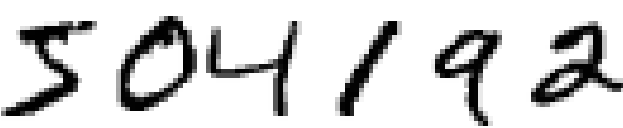
\includegraphics{504192}
%     \end{marginfigure}

\begin{figure*}[h]
    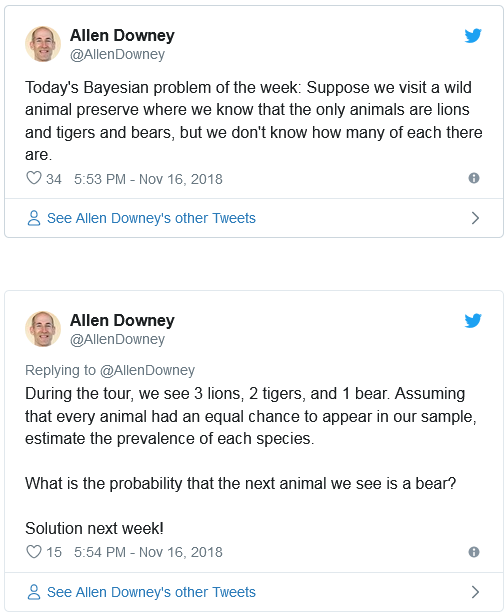
\includegraphics[width=0.56\textwidth]{p05c02-snip01}
    \caption{Allen Downey tweets}
    \label{fig:p05c02-snip01}
    \end{figure*}


This may seem like a simple problem --- the prevalences are simply the same as the observed data (50\% lions, 33\% tigers and 17\% bears) right? If you believe observations we make are a perfect representation of the underlying truth, then yes, this problem could not be easier. However, as a Bayesian \cite{RationalWikiBayesian2019}, this view of the world and the subsequent reasoning is deeply unsatisfying.

First, how can we be sure this single trip to the preserve was indicative of all trips? What if we went during the winter when the bears were hibernating? We need to include uncertainty in our estimate considering the limited data. Second, how can we incorporate prior beliefs about the situation into this estimate? If we have heard from a friend the preserve has an equal number of each animal, then surely this should play some role in our estimate.

\textit{Fortunately, there is a solution that allows to express uncertainty and incorporate prior information into our estimate: Bayesian Inference.}

In this article, we'll explore the problem of estimating probabilities from data in a Bayesian framework, along the way learning about probability distributions, 
Bayesian Inference \cite{wikipediaBayesianinference2019}, and 
basic probabilistic programming \cite{CameronDavidsonPilonGitHub2019} \cite{CameronDavidsonPilonBlog2019} 
with PyMC3 \cite{PyMC3API2019}. The complete code is available as a Jupyter Notebook on GitHub \cite{KoehrsenEstiBayesGithub2018}.

    \begin{figure*}[h]
        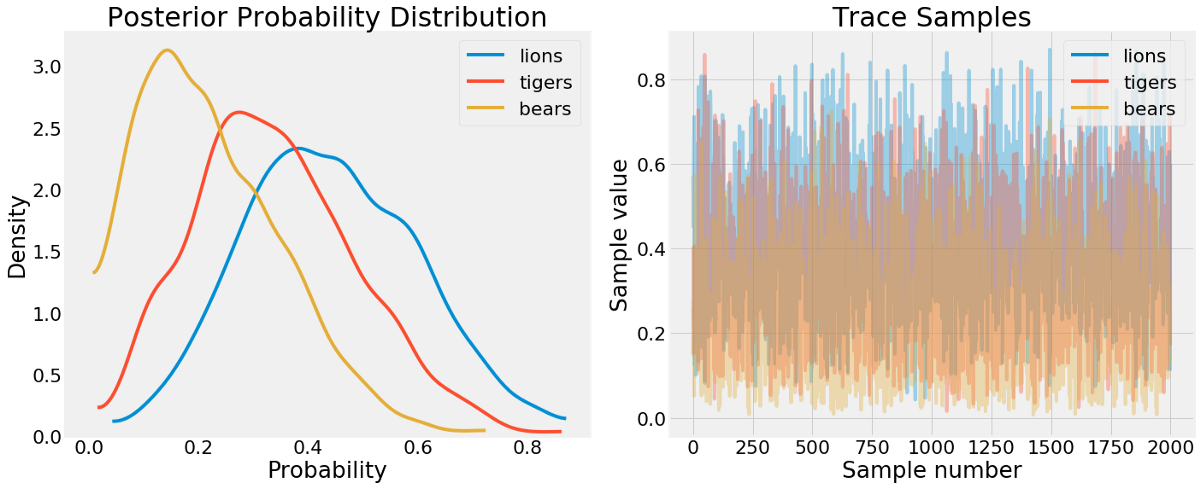
\includegraphics[width=0.56\textwidth]{p05c02-snip02}
        \caption{PDF and trace values from PyMC3}
        \label{fig:p05c02-snip02}
        \end{figure*}
    
\section{Background Concepts}

Often, especially in statistics, I find the theory behind a solution \textit{more confusing} than actually solving the problem. (I'm convinced statisticians complicate statistics to justify their existence.) Coding an answer and visualizing the solution usually does more for me than reading endless equations. Therefore, when I approached this problem, I studied just enough of the ideas to code a solution, and only \textit{after} did I dig back into the concepts.

This reflects my general \textit{top-down} \cite{RachelThomas2019} approach to learning new topics. Instead of starting with the fundamentals --- which are usually tedious and difficult to grasp --- find out how to implement an idea so you know \textit{why it's useful} and then go back to the formalisms. So, if you feel yourself getting frustrated with the theory, move on to the solution (starting with the Inference section below), and then come back to the concepts if you're still interested.

(This top-down philosophy is exemplified in the excellent fast.ai courses on deep learning \cite{RachelThomas2019}. These courses, besides effectively teaching neural networks, have been influential in my approach to learning new techniques.)

\section{Bayesian Model}

Since we want to solve this problem with Bayesian methods, we need to construct a model of the situation. The basic set-up is we have a series of observations: 3 tigers, 2 lions, and 1 bear, and from this data, we want to estimate the prevalence of each species at the wildlife preserve. That is, we are looking for the posterior probability of seeing each species given the data.

Before we begin we want to establish our assumptions:


\begin{itemize}
\item Treat each observation of one species as an independent trial.
\item Our initial (prior) belief is each species is equally represented.
\end{itemize}

The overall system, where we have 3 \textbf{discrete} choices (species) each with an unknown probability and 6 total observations is a\textbf{ multinomial distribution}. The multinomial distribution is the extension of the binomial distribution to the case where there are more than 2 outcomes. A simple application of a multinomial is 5 rolls of a dice each of which has 6 possible outcomes.

A probability mass function \cite{WikipeadiaProbabilitymassfunction2019} of a multinomial with 3 discrete outcomes is shown in the figure.

\begin{marginfigure}
    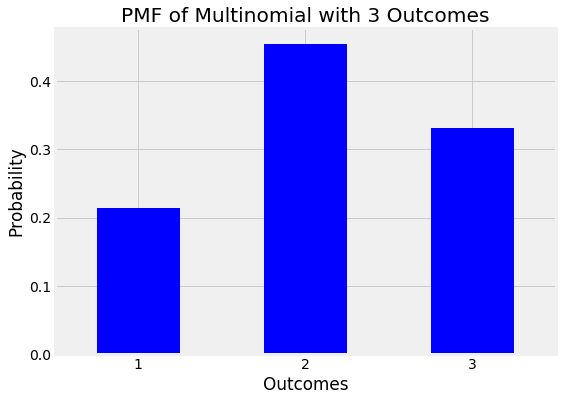
\includegraphics{p05c02-snip03}
    \caption{Probability Mass Function (PMF) of a multinomial with 3 outcomes}
    \end{marginfigure}

A Multinomial distribution is characterized by $k$, the number of outcomes, $n$, the number of trials, and 
$\mathbf {p}$, a vector of probabilities for each of the outcomes. For this problem, $\mathbf {p}$ is our ultimate objective: we want to figure out the probability of seeing each species from the observed data. In Bayesian statistics, the parameter vector for a multinomial is drawn from a \textbf{Dirichlet Distribution}, which forms the prior distribution for the parameter.

The Dirichlet Distribution, in turn, is characterized by, $k$, the number of outcomes, and  $\boldsymbol {\alpha }$, a vector of positive real values called the concentration parameter. This is called a \textbf{hyperparameter} because it is a \textit{parameter of the prior}. (This chain can keep going: if  $\boldsymbol {\alpha }$ comes from another distribution then this is a \textit{hyperprior} which could have its \textit{own parameters} called \textit{hyperyhyperparameters}!). We'll stop our model at this level by explicitly setting the values of $\boldsymbol {\alpha }$, which has one entry for each outcome.

\section{Hyperparameters and Prior Beliefs}

The best way to think of the Dirichlet parameter vector is as pseudocounts, observations of each outcome that occur before the actual data is collected. These pseudocounts \textit{capture our prior belief about the situation}. For example, because we think the prevalence of each animal is the same before going to the preserve, we set all of the $\alpha_i $ values to be equal, say  $\boldsymbol {\alpha }$ = [1, 1, 1].

Conversely, if we expected to see more bears, we could use a hyperparameter vector like [1, 1, 2] (where the ordering is [lions, tigers, bears]. The exact value of the pseudocounts reflects the level of confidence we have in our prior beliefs. Larger pseudocounts will have a greater effect on the posterior estimate while smaller values will have a smaller effect and will let the data dominate the posterior. We'll see this when we get into inference, but for now, remember that the hyperparameter vector is pseudocounts, which in turn, represent our prior belief.

A Dirichlet distribution with 3 outcomes is shown below \cite{FrancisTsengBayesianLearning2019} with different values of the hyperparameter vector. Color indicates the concentration weighting.

    \begin{figure*}[h]
        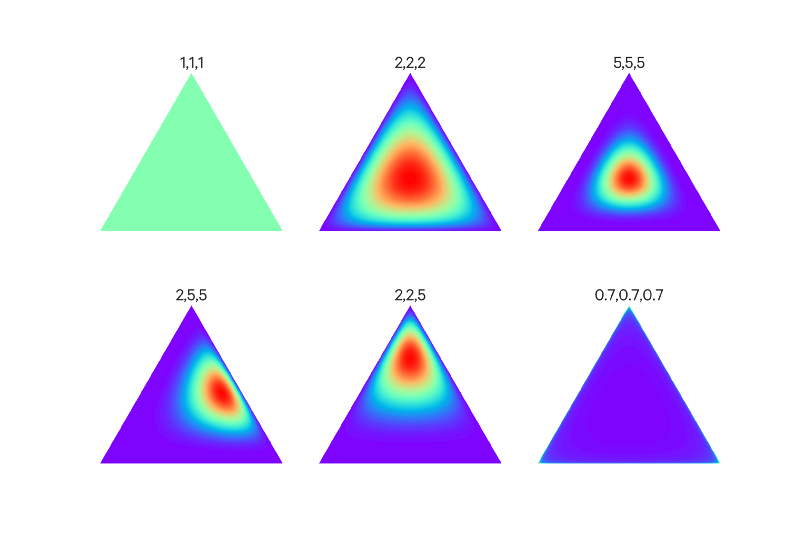
\includegraphics[width=0.8\textwidth]{p05c02-snip04}
        \caption{Effect of the hyperparameter vector $\boldsymbol {\alpha }$ on the Dirichlet Distribution}
    \end{figure*}

There's a lot more detail we don't need to get into here, but if you're still curious, see some of the sources listed below.

Our ultimate goal is to estimate the posterior distribution for the probability of observing each species, $\mathbf {p}$, conditioned on the data and hyperparameters. The posterior distribution of the parameter is our objective. $\mathbb {X}$ is observations and $\boldsymbol {\alpha }$ is hyperparameters.

\begin{equation}
    \mathbf {p}\mid \mathbb {X} ,{\boldsymbol {\alpha }}
\end{equation}

Our final model, consisting of a multinomial distribution with Dirichlet priors is called a Dirichlet-Multinomial and is visualized below:

\begin{figure*}[h]
    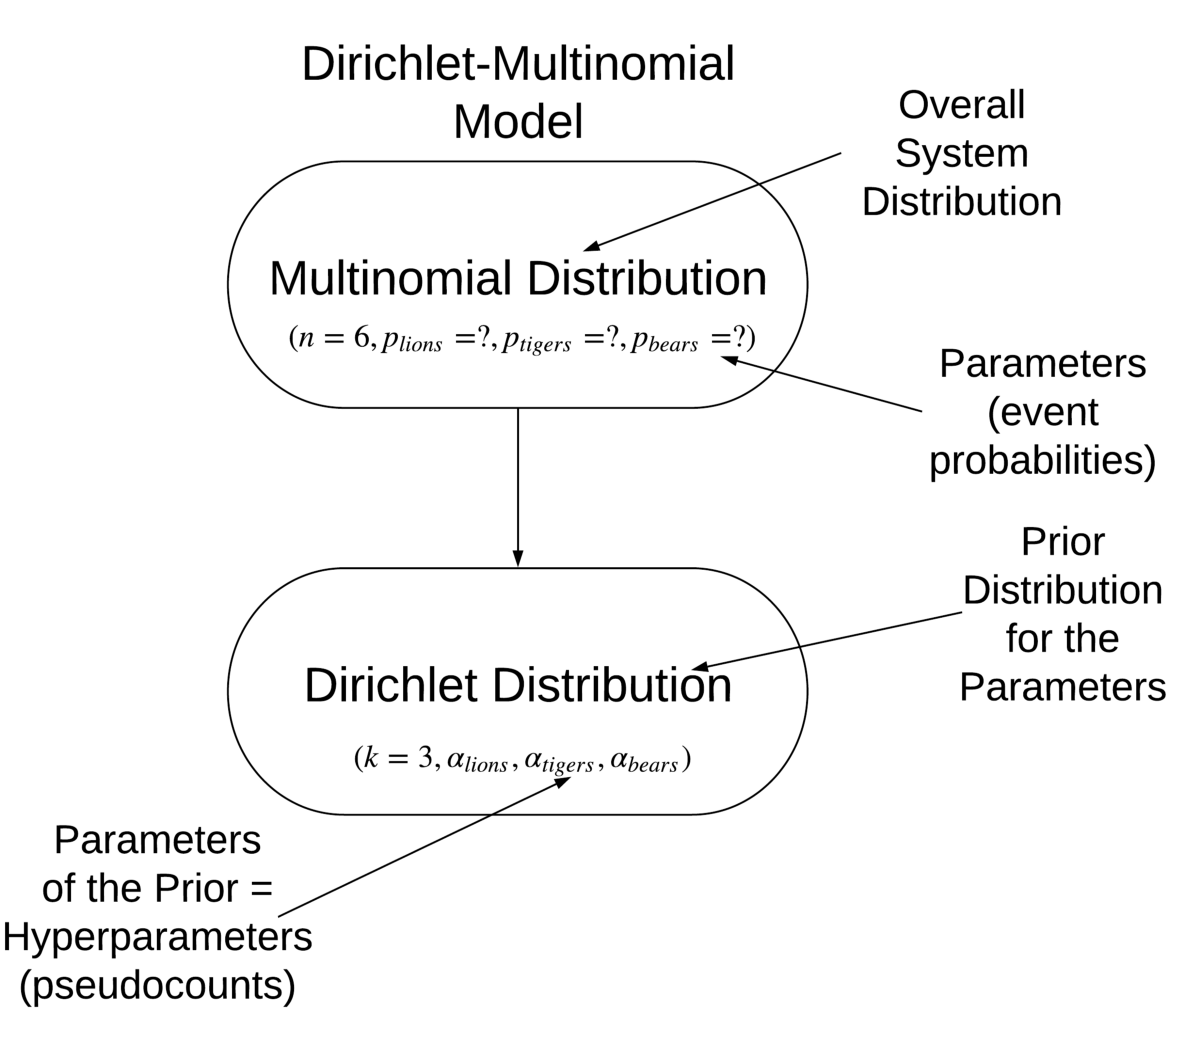
\includegraphics[width=0.5\textwidth]{p05c02-snip05}
    \caption{Model of the problem}
\end{figure*}

A summary of the problem specifics is below:

\begin{figure*}[h]
    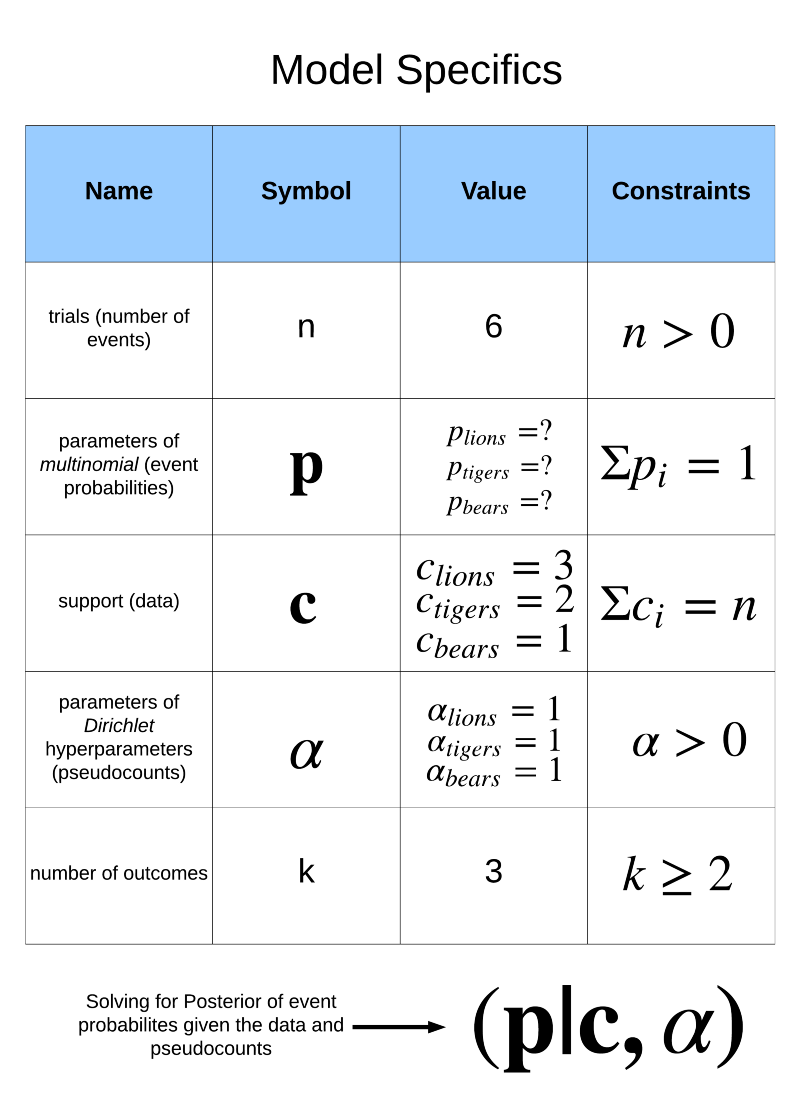
\includegraphics[width=0.5\textwidth]{p05c02-snip06}
    \caption{Model specifics}
\end{figure*}


If you still want more background details, here are some of the sources I relied on (the first is probably the most valuable):

Sources:


\begin{enumerate}
\item Bayesian Inference for Dirichlet-Multinomials \cite{MarkJohnsonDirichletMultinomials2019}.
\item Categorical Data / Multinomial Distribution \cite{ChristianHertaCategoricaldata2019}.
\item Dirichlet-Multinomial Wikipedia Article \cite{WikiPediaDirichletmultinomial2019}.
\item Multinomial Distribution Wikipedia Article \cite{WikiPediaMultinomialdistribution2019}.
\item Alpha in the Dirichlet Distribution \cite{stackexchangealphaDirichlet2019}.
\item Dirichlet Distribution Wikipedia Article \cite{WikiPediaDirichletdistributionl2019}.
\item Hyperparameter Wikipedia Article \cite{WikiPediaHyperparameter2019}.
\item Deriving the MAP estimate for Dirichlet-Multinomials \cite{stackexchangeMAPMultinomialDirichlet2019}.
\end{enumerate}

There are also other ways to approach this problem; see here for Allen Downey's solution \cite{AllenBDowneyThinkBayes2018} which yields similar results.

\section{Inference: Making Estimates from Data}

Now that we have the model of the problem, we can solve for the posteriors using Bayesian methods. Inference in statistics is the process of estimating (inferring) the unknown parameters of a probability distribution from data \cite{WikiPediaStatisticalinference2019}. Our unknown parameters are the prevalence of each species while the data is our single set of observations from the wildlife preserve. Our goal is to find the posterior distribution of the probability of seeing each species.

Our approach to deriving the posterior will use Bayesian inference. This means we build the model and then use it to \textit{sample from the posterior to approximate the posterior} with Markov Chain Monte Carlo (MCMC) methods \cite{KoehrsenMCMCPython2018}. We use MCMC when exact inference is intractable, and, as the number of samples increases, the estimated posterior converges to the true posterior.

The result of MCMC is not just one number for our answer, but rather a range of samples that lets us quantify our uncertainty especially with limited data. We'll see how to perform Bayesian inference in Python shortly, but if we do want a single estimate, we can use the \textit{Expected Value} of the distribution.

\section{Expected Value}

The Expected Value is the mean of the posterior distribution. For a Dirichlet-Multinomial priors, the expected value  can be analytically expressed \cite{MarkJohnsonDirichletMultinomials2019}:
\begin{equation}
    \mathrm{E}\left[p_{i} | \mathbb{X}, \boldsymbol{\alpha}\right]=\frac{c_{i}+\alpha_{i}}{N+\sum_{k} \alpha_{k}}
    \end{equation}

Once we start plugging in numbers, this becomes easy to solve. N is the number of trials, 6, $c_i$ is the \textit{observed count} for each category, and $alpha_i$ is the \textit{pseudocount} (hyperparameter) for each category. Setting all $\boldsymbol{\alpha}$ equal to 1, the expected species probabilities can be calculated:

\begin{lstlisting}
species = ['lions', 'tigers', 'bears']
# Observations
c = np.array([3, 2, 1])
#Pseudocounts
alphas = np.array([1, 1, 1])

expected = (alphas + c) / (c.sum() + alphas.sum())

Species: lions    Prevalence: 44.44%.
Species: tigers   Prevalence: 33.33%.
Species: bears    Prevalence: 22.22%.
\end{lstlisting}
This represents the expected value taking into account the pseudocounts which corporate our initial belief about the situation.

We can adjust our level of confidence in this prior belief by increasing the magnitude of the pseudocounts. This forces the expected values closer to our initial belief that the prevalence of each species is equal. The expected values for several different hyperparameters are shown below:


\begin{figure*}[h]
    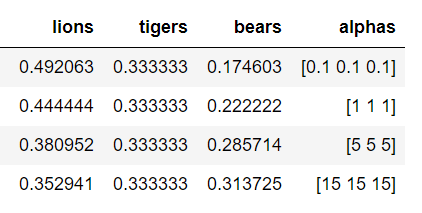
\includegraphics[width=0.5\textwidth]{p05c02-snip07}
    \caption{Expected values for different pseudocounts}
\end{figure*}

Our choice of hyperparameters has a large effect. If we are more confident in our belief, then we increase the weight of the hyperparameters. On the other hand, if we want the data to have more weight, we reduce the pseudocounts.

While this result provides a point estimate, it's misleading because it does not express any uncertainty. We only went to the wildlife preserve once, so there should be a large amount of uncertainty in these estimates. With Bayesian Inference, we can get both point estimates and the uncertainty.

\section{Bayesian Inference in Python with PyMC3}

To get a range of estimates, we use Bayesian inference by constructing a model of the situation and then \textit{sampling from the posterior to approximate the posterior}. This is implemented through Markov Chain Monte Carlo (or a more efficient variant called the No-U-Turn Sampler) \cite{Hoffman:2014:NSA:2627435.2638586} in PyMC3. Compared to the theory behind the model, setting it up in code is simple:


\begin{lstlisting}
    import pymc3 as pm
    import numpy as np
    
    alphas = np.array([1, 1, 1])
    c = np.array([3, 2, 1])
    
    # Create model
    with pm.Model() as model:
        # Parameters of the Multinomial are from a Dirichlet
        parameters = pm.Dirichlet('parameters', a=alphas, shape=3)
        # Observed data is from a Multinomial distribution
        observed_data = pm.Multinomial(
            'observed_data', n=6, p=parameters, shape=3, observed=c)   
    
\end{lstlisting}

Then, we can sample from the posterior:

\begin{lstlisting}
    with model:
        # Sample from the posterior
        trace = pm.sample(draws=1000, chains=2, tune=500, 
                          discard_tuned_samples=True)
\end{lstlisting}

This code draws 1000 samples from the posterior in 2 different chains (with 500 samples for tuning that are discarded). We are left with a trace which contains all of the samples drawn during the run. We use this trace to estimate the posterior distribution.

PyMC3 has many methods for inspecting the trace such as \lstinline{pm.traceplot} (Figure~\ref{fig:p05c02-snip02b}).

\begin{figure*}[h]
    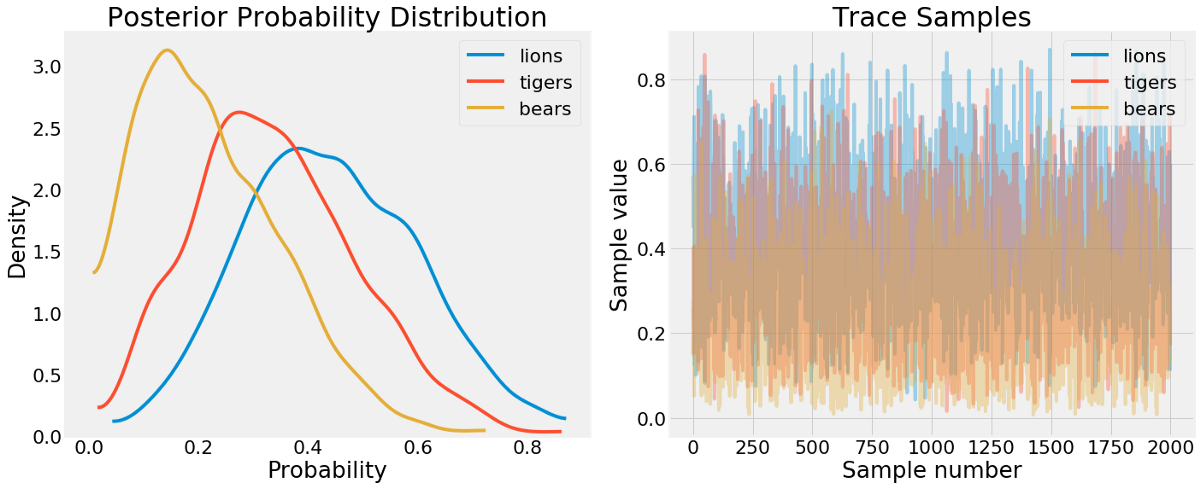
\includegraphics[width=0.5\textwidth]{p05c02-snip02}
    \caption{PDF and trace of samples}
    \label{fig:p05c02-snip02b}
\end{figure*}

On the left we have a kernel density estimate for the sampled parameters --- a PDF of the event probabilities. On the right, we have the complete samples drawn for each free parameter in the model. We can see from the KDE that $p_\textrm{bears}<p_\textrm{tigers}<p_\textrm{lions}$ as expected but there is some uncertainty. A better way to view this uncertainty is through \lstinline{pm.posterior_plot} (Figure~\ref{fig:p05c02-snip09}).

\begin{figure*}[h]
    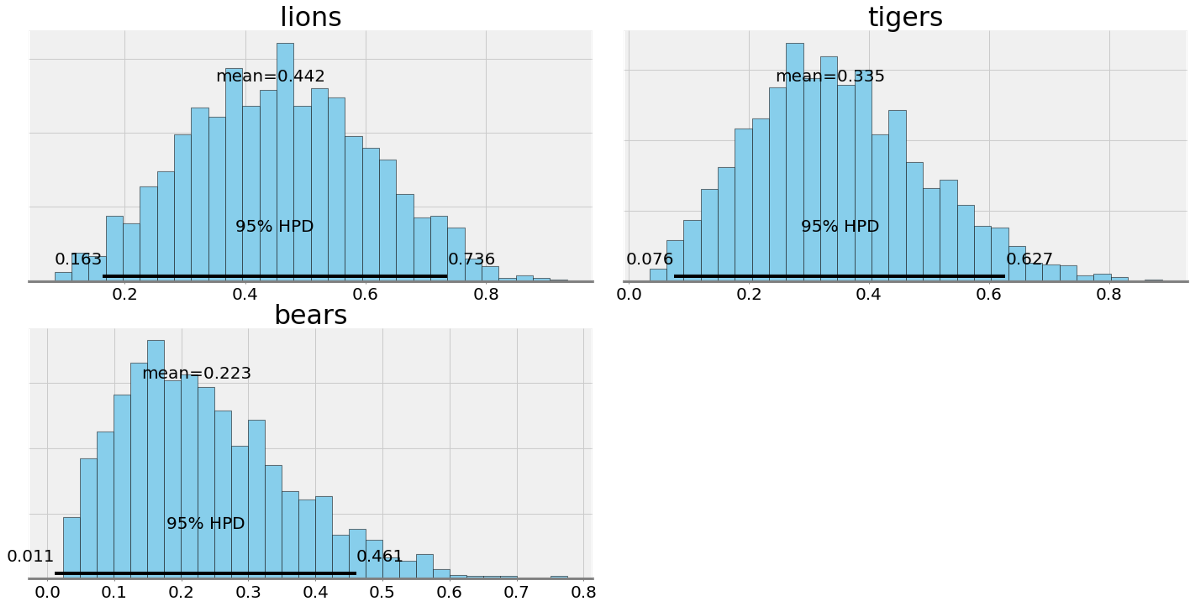
\includegraphics[width=0.5\textwidth]{p05c02-snip09}
    \caption{Posterior plots from PyMC3}
    \label{fig:p05c02-snip09}
\end{figure*}

Figure~\ref{fig:p05c02-snip09} shows histograms indicating the number of times each probability was sampled from the posterior. We have a point estimate for the probabilities --- the mean --- as well as the Bayesian equivalent of the confidence interval --- the 95\% highest probability density (also known as a credible interval). We see an extreme level of uncertainty in these estimates, as befits the limited data.

To quantify the level of uncertainty we can get a dataframe of the results:

\begin{figure*}[h]
    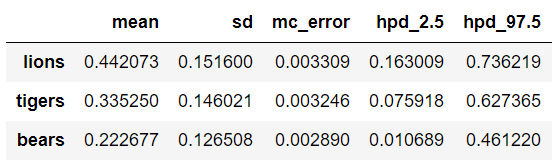
\includegraphics[width=0.5\textwidth]{p05c02-snip10}
    \caption{Posterior plots from PyMC3}
\end{figure*}

This shows the best estimate (mean) for the prevalence but also that the 95\% credible interval is very large. We can only nail down the prevalence of lions to between 16.3\% and 73.6\% based on our single trip to the preserve!

Bayesian Inference is so powerful because of this built-in uncertainty. In the real-world, data is always noisy, and we usually have less than we want. Therefore, any time we make an estimate from data we have to show this uncertainty. For this problem, no one is going to be hurt if we get the percentage of bears at the wildlife preserve incorrect, but what if we were doing a similar method with medical data and inferring disease probability?

\section{Sampling from the Posterior}

Once we have the trace, we can draw samples from the posterior to simulate additional trips to the preserve. For example, let's consider going 1000 more times. How many of each species can we expect to see on each trip?



\begin{lstlisting}
    # Sample from the posterior
    with model:
        samples = pm.sample_ppc(trace, samples = 1000)
\end{lstlisting}

\begin{figure*}[h]
    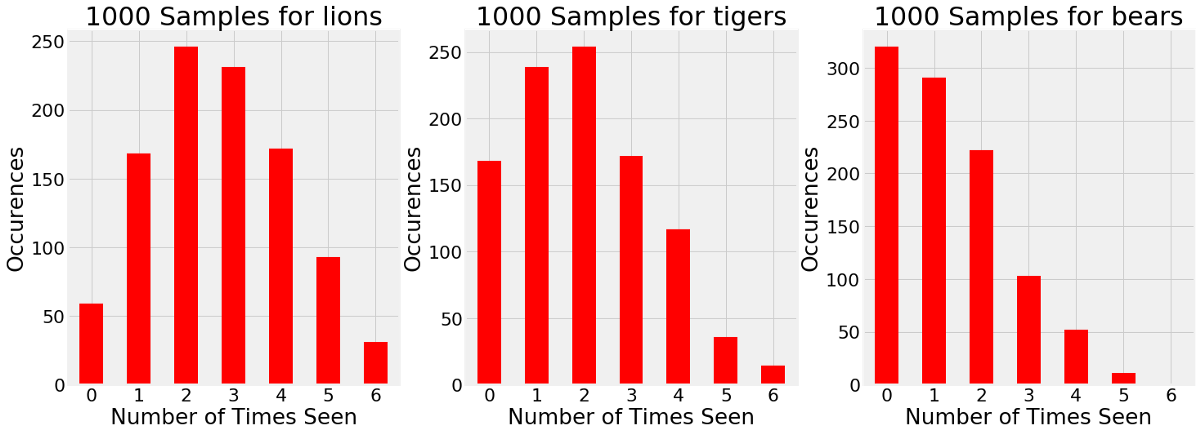
\includegraphics[width=0.5\textwidth]{p05c02-snip11}
    \caption{1000 samples drawn from the estimated posterior}
\end{figure*}

Based on the evidence, there are times when we go to the preserve and see 5 bears and 1 tiger! Granted, this is not very likely, graphs such as these show the entire range of possible outcomes instead of only one. Our single trip to the preserve was just one outcome: 1000 simulations show that we can't expect the exact observations every time we go to the preserve.

If we want to see the new Dirichlet distribution after sampling, it looks like:

\begin{figure*}[h]
    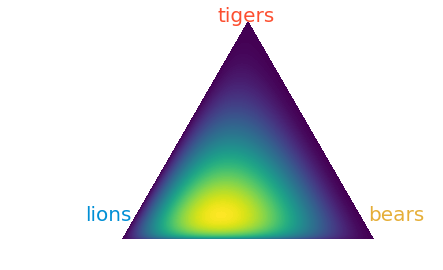
\includegraphics[width=0.3\textwidth]{p05c02-snip12}
    \caption{Dirichlet distribution after sampling}
\end{figure*}


\section{Incorporating Additional Information}

What happens when we go 4 times to the preserve and want to incorporate additional observations in our model? In PyMC3, this is simple:

\begin{lstlisting}
    # Observations from multiple trips
    c = np.array([[3, 2, 1],
                  [2, 3, 1],
                  [3, 2, 1],
                  [2, 3, 1]])
    
    with pm.Model() as model:
        # Parameters are a dirichlet distribution
        parameters = pm.Dirichlet('parameters', a=alphas, shape=3)
        # Observed data is a multinomial distribution
        observed_data = pm.Multinomial(
            'observed_data', n=6, p=parameters, shape=3, observed=c)    
        
        trace = pm.sample(draws=1000, chains=2, tune=500, discard_tuned_samples=True)
\end{lstlisting}

The uncertainty in the posterior should be reduced with a greater number of observations, and indeed, that is what we see both quantitatively and visually. Intuitively, this again makes sense: as we gather more data, we become more sure of the state of the world. In the case of infinite data, our estimate will converge on the true values and the priors will play no role.

\begin{figure*}[h]
    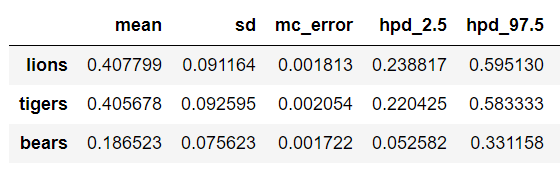
\includegraphics[width=0.5\textwidth]{p05c02-snip13}
\end{figure*}
\begin{figure*}[h]
    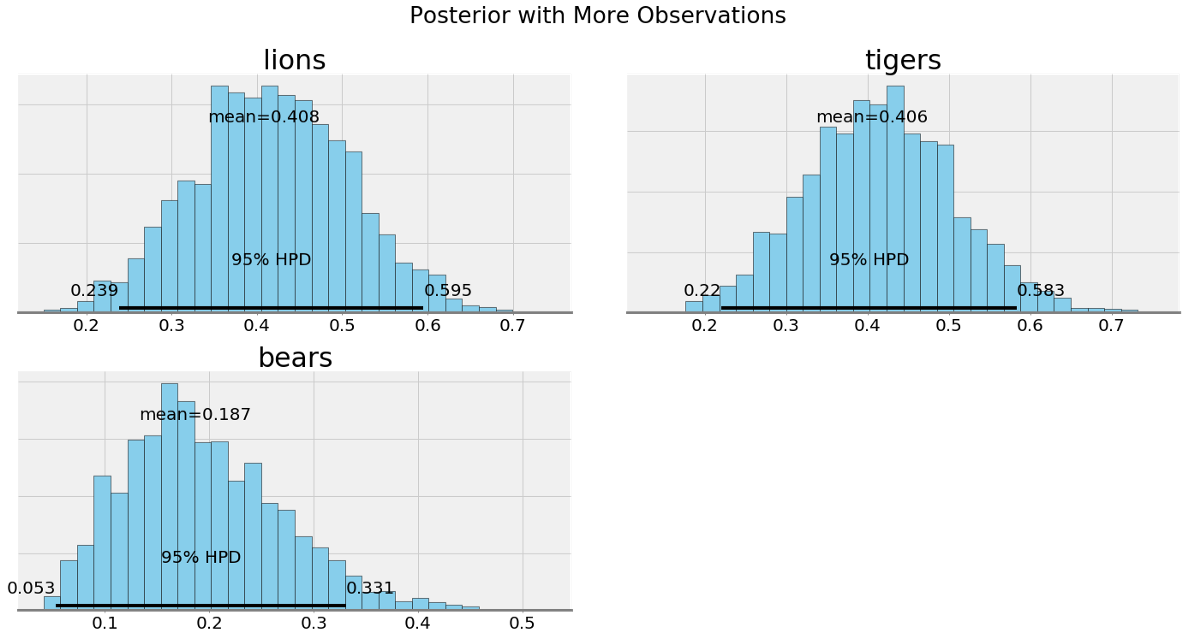
\includegraphics[width=0.5\textwidth]{p05c02-snip14}
    \caption{Posteriors with more data}
\end{figure*}


\section{Increasing and Decreasing Confidence in Prior Beliefs}

Earlier we discussed how the hyperparameters can be thought of as pseudocounts that represent our prior belief. If we set all the values of $\bm \alpha$ equal to 1, we get the results we've seen so far. What about if we decrease or increase our confidence in our initial theory that the prevalence is equal? To do so, all we have to do is alter the $\boldsymbol {\alpha }$ vector. Then, we sample from the posterior again (using the original observations) and inspect the results.

\begin{figure*}[h]
    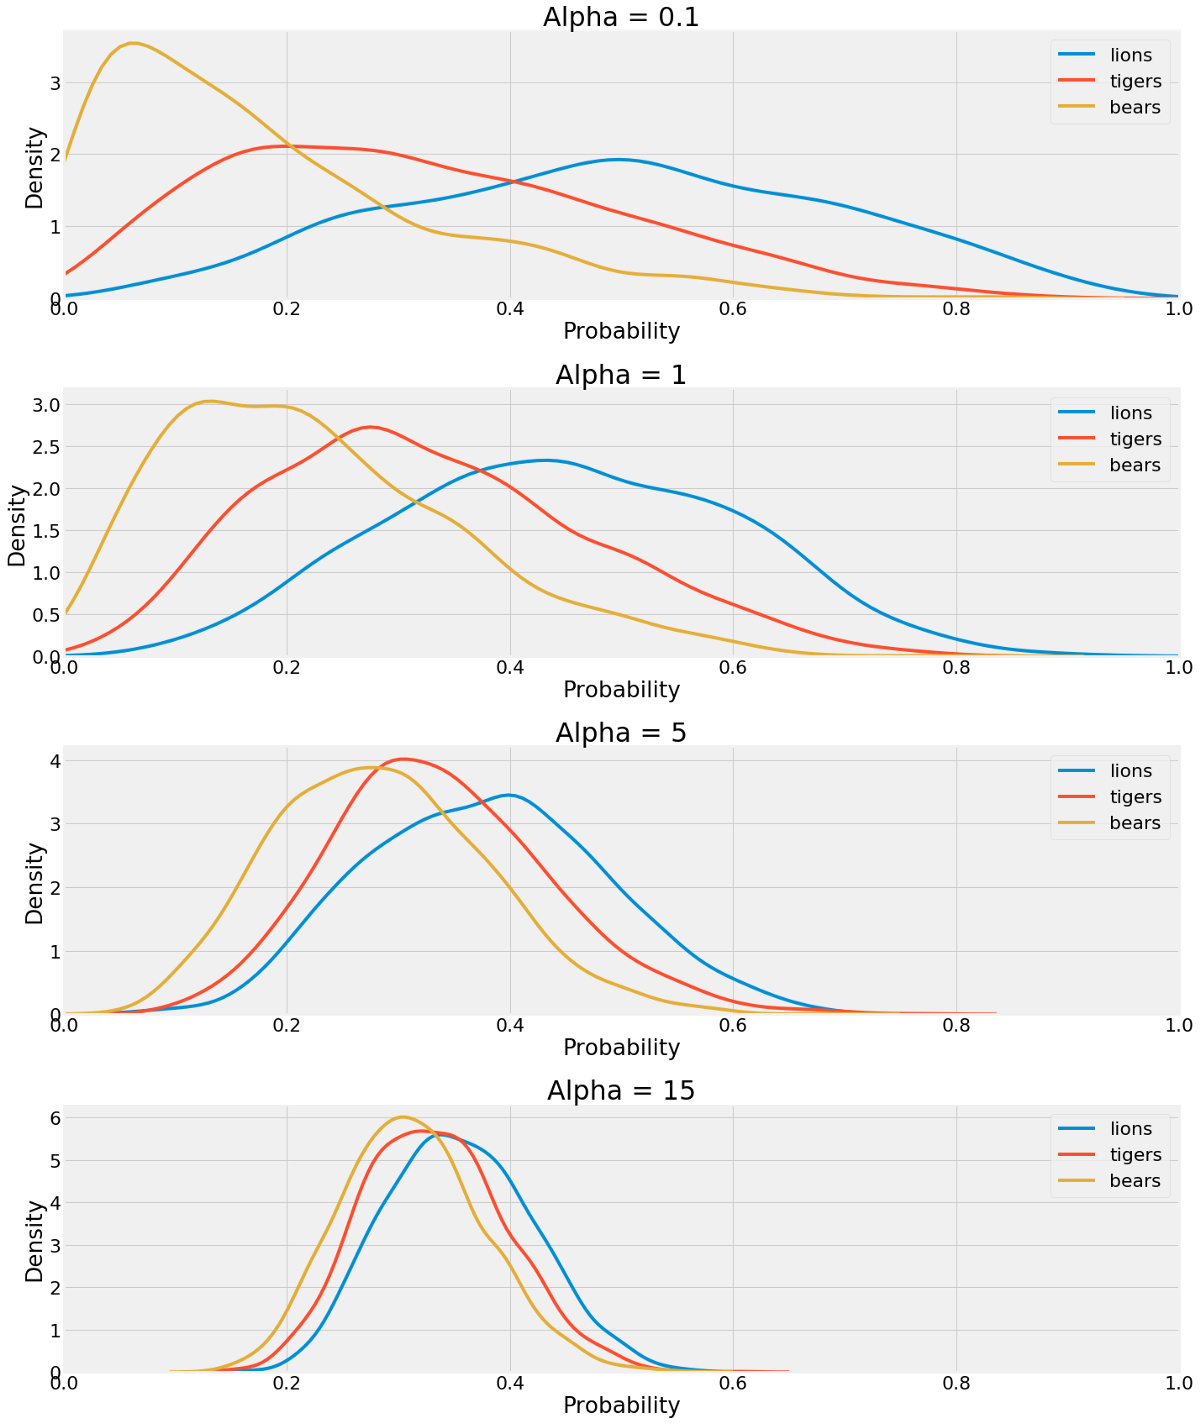
\includegraphics[width=0.7\textwidth]{p05c02-snip15}
\end{figure*}



The hyperparameters have a large influence on the outcome! A lower value means the data itself has a greater weighting in the posterior, while a higher value results in greater weight placed on the pseudocounts. As the value is increased, the distributions converge on one another. We'd need a lot of data to overcome our strong hyperparameters in the last case.

We can compare the posterior plots with $\bm \alpha$ = 0.1 and $\bm \alpha$ = 15 in Figure~\ref{fig:p05c02-snip16}.


\begin{figure*}[h]
    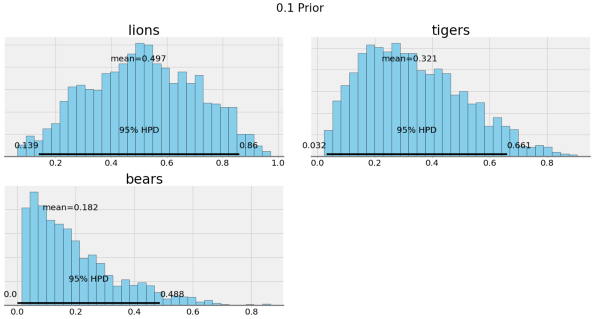
\includegraphics[width=0.7\textwidth]{p05c02-snip16}\\
    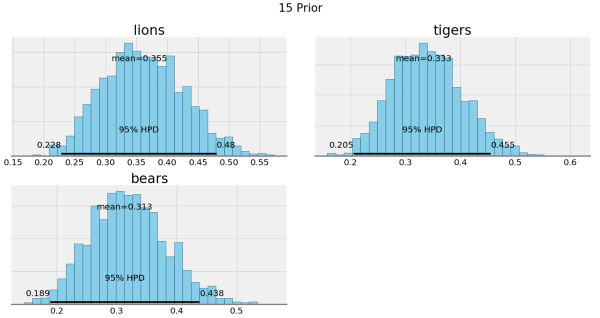
\includegraphics[width=0.7\textwidth]{p05c02-snip17}
    \caption{Posterior plots with different $\bm \alpha$ }
    \label{fig:p05c02-snip16}
\end{figure*}


Ultimately, our choice of the hyperparameters depends on our confidence in our belief. If we have a good reason to think the prevalence of species is equal, then we should make the hyperparameters have a greater weight. If we want to let the data speak, then we can lower the effect of the hyperparameters.

\FloatBarrier
\section{Conclusions}

Well, what should our final answer be to the question of prevalences? If we are good Bayesians, then we can present a point estimate, but only with attached uncertainty (95\% credible intervals):

\begin{lstlisting}
    Lions: 44.5% (16.9% --- 75.8%)
    Tigers: 32.7% (6.7% --- 60.5%)
    Bears: 22.7% (1.7% --- 50.0%)
\end{lstlisting}
And our estimate that the next observation is a bear? Based on the posterior sampling, about 23\%. While these results may not be satisfying to people who want a simple answer, they should remember that the real world is uncertain.

The benefits of Bayesian Inference \cite{RStatModCausalRisks2019} are we can incorporate our prior beliefs and we get uncertainty estimates with our answers. The world is uncertain, and, as responsible data scientists, Bayesian methods provide us with a framework for dealing with uncertainty.

Furthermore, as we get more data, our answers become more accurate. As with many aspects of Bayesian Inference, this is in line with our intuitions and how we naturally go about the world, becoming less wrong with additional information. Ultimately, Bayesian statistics is enjoyable and useful because it is statistics that finally makes sense.

As always, I welcome feedback and constructive criticism. I can be reached on Twitter \lstinline{@koehrsen_will} or through my personal website \lstinline{willk.online}.
